%\chapter{Obsah CD}
\chapter{Inštalácia}
{
	V tejto kapitole by som Vád objasnil postup inštalácie aplikácie. V prvom rade uviediem potrebné prostriedky pre beh aplikácie. Pre správny beh aplikácie potrebujeme nasledovné prostriedky:
	\begin{itemize}
	\item JBoss aplikačný server najmenej vo verzii 7.1.1.Final. Je možné ho zdarma stiahnuť z www.jboss.org
	\item Nástroj Maven, ktorý je možné stiahnuť vo verzii 3.2.1 z www.maven.apache.org, kde sa nachádza aj manuál na inštaláciu
	\item MySQL Connector/J minimálne vo verzii 5.0.8, ktorý môžte stiahnuť z https://dev.mysql.com/downloads/connector/j/
	\item MySQL databázový server najmenej vo verzii 5.5.37
	\item Webový prehlidač Mozilla Firefox najmenej vo verzii 29.0 alebo Google Chrome najmenej vo verzii 34.0
	\end{itemize}
	V prvom rade je potrebné nainštalovať MySQL server nakonfigurovať databázu s názvom \uv{optaplanner} s užívateľským menom \uv{root} a heslom \uv{root}. Následne je potrebné rozbaliť JBoss aplikačný server na súborový systém. V ďalšom kroku nastaví náš aplikačný server pre správne použitie MySQL databáze. V tomto kroku je potrebné nakonfigurovať súbor \emph{standalone.xml} v adresári JBOSS_HOME/standalone/configuration/. Tam správne nastavíme datasource(zdroj databázových dát pre našlu aplikáciu)(môžme použiť online dokumentáciu https://docs.jboss.org/author/display/AS71/DataSource+configuration, kde je celý postup zdokumentovaný). Následne treba stiahnutý MySQL Connector/J skopírovať do adresára JBOSS_HOME/standalone/deployments. Aplikáciu môžme spustiť nasledovne:
	\begin{itemize}
	\item Skopírujeme maven projekt optaplanner.controller do adresára JBOSS_HOME/standalone/deployments
	\item Skopírujeme maven projekt PlannerService do adresára JBOSS_HOME/standalone/deployments
	\item Prejdeme do zložky JBOSS_HOME/standalone/bin a spustíme skript \emph{standalone.sh}
	\end{itemize}
	Aplikáciu je možné spustiť aj pomocou nástroju maven a to nasledovne:
	\begin{itemize}
	\item Nastavíme sa na projekt optaplanner.controller a zadamé príkaz mvn package
	\item Následne zadamé príkaz mvn compile
	\item A nakoniec príkaz mvn jboss as:deploy
	\end{itemize}
	Postup uvedený vyššie vykonáme aj pre projekt Planner.Service. 
	Aplikáciu spustíme zadaním príkazu \uv{http://localhost:8080/optaplanner.controller/} do webového prehliadaču.


}

\chapter{Užívatelské rozhranie}
{
	\begin{figure}[htb]

\begin{center}

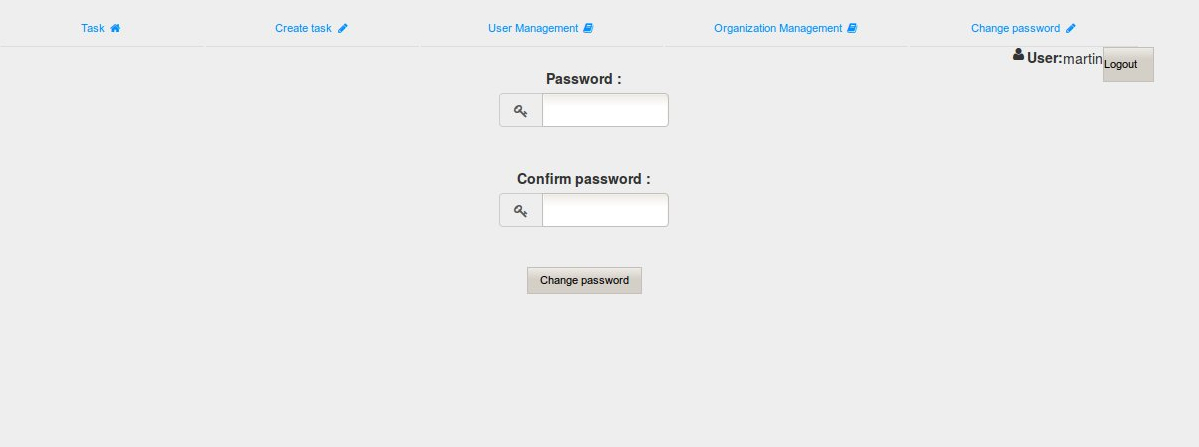
\includegraphics[scale=0.5]{page5.jpg} 
\caption{Prihlasovacia obrazovka }


\end{center}

\end{figure}


\begin{figure}[htb]

\begin{center}

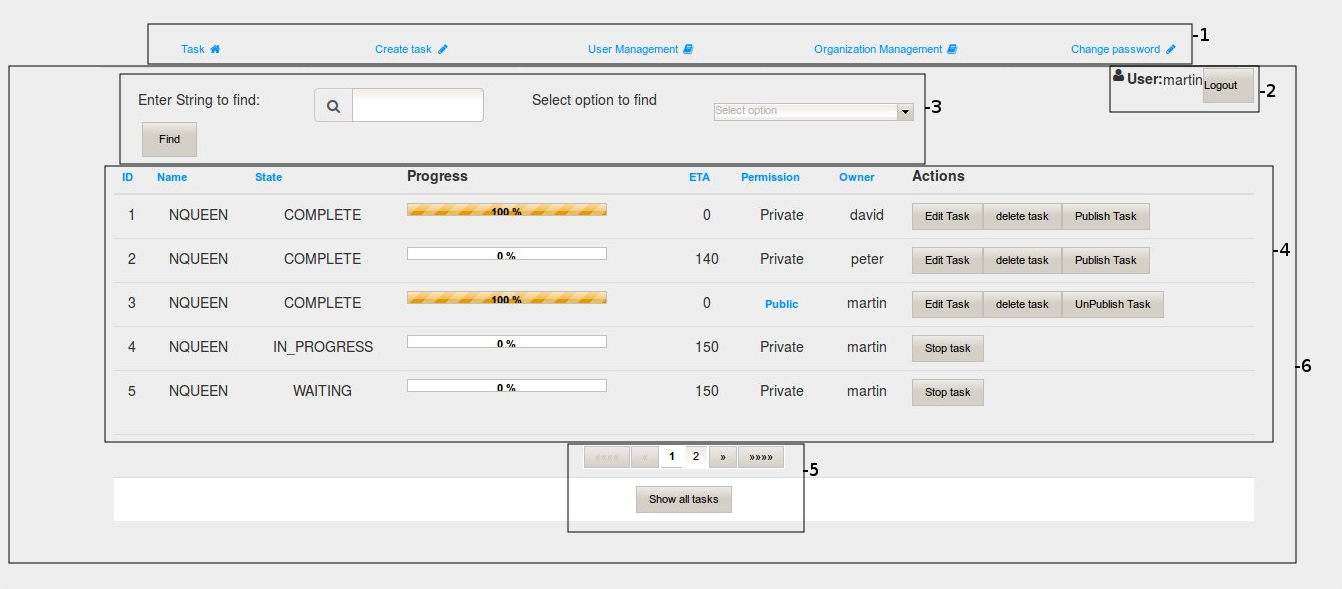
\includegraphics[scale=0.5]{page.jpg} 
\caption{Zobrazenie úloh spolu s akciami }


\end{center}

\end{figure}



\begin{figure}[htb]

\begin{center}

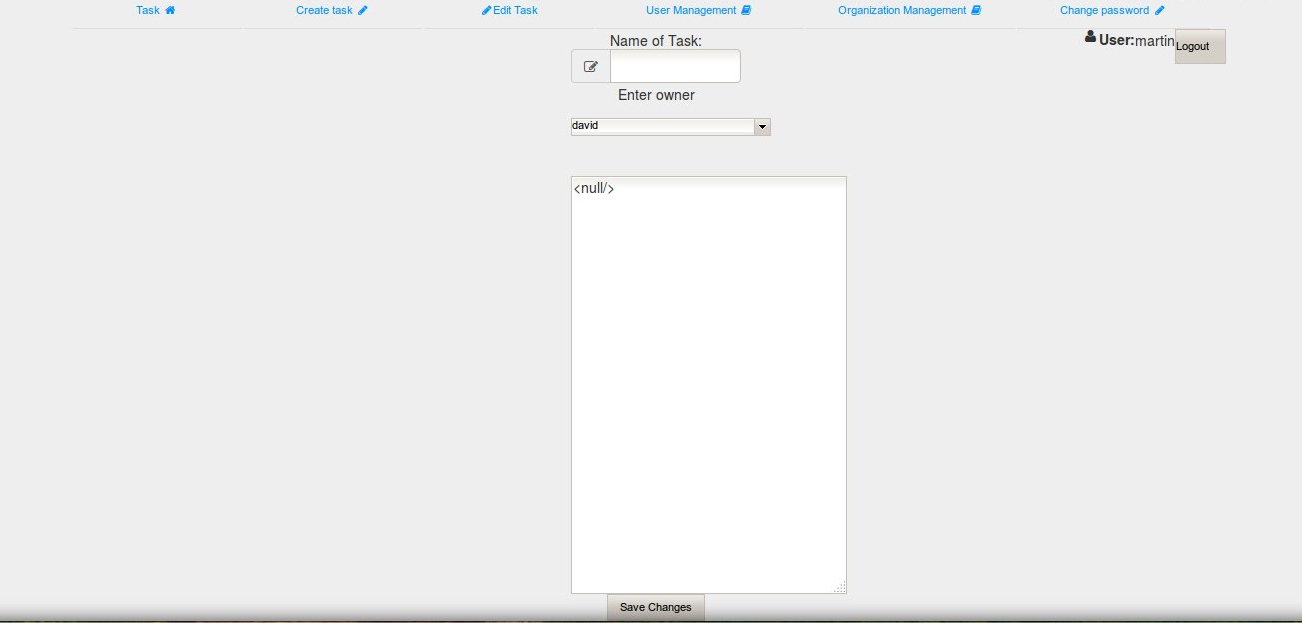
\includegraphics[scale=0.5]{page1.jpg} 
\caption{Nahrávanie novej úlohy}


\end{center}

\end{figure}

\begin{figure}[htb]

\begin{center}

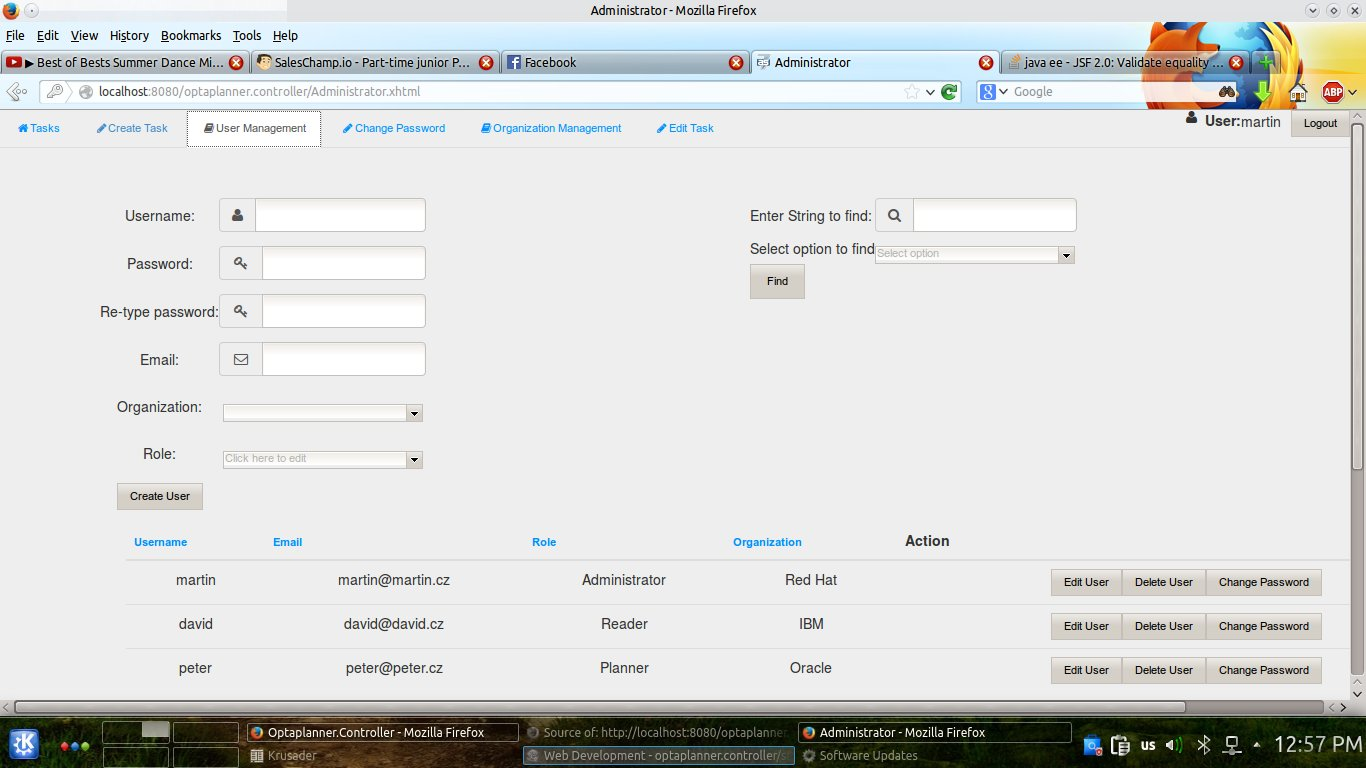
\includegraphics[scale=0.5]{page2.jpg} 
\caption{Spravovanie užívateľov}


\end{center}

\end{figure}


\begin{figure}[htb]

\begin{center}

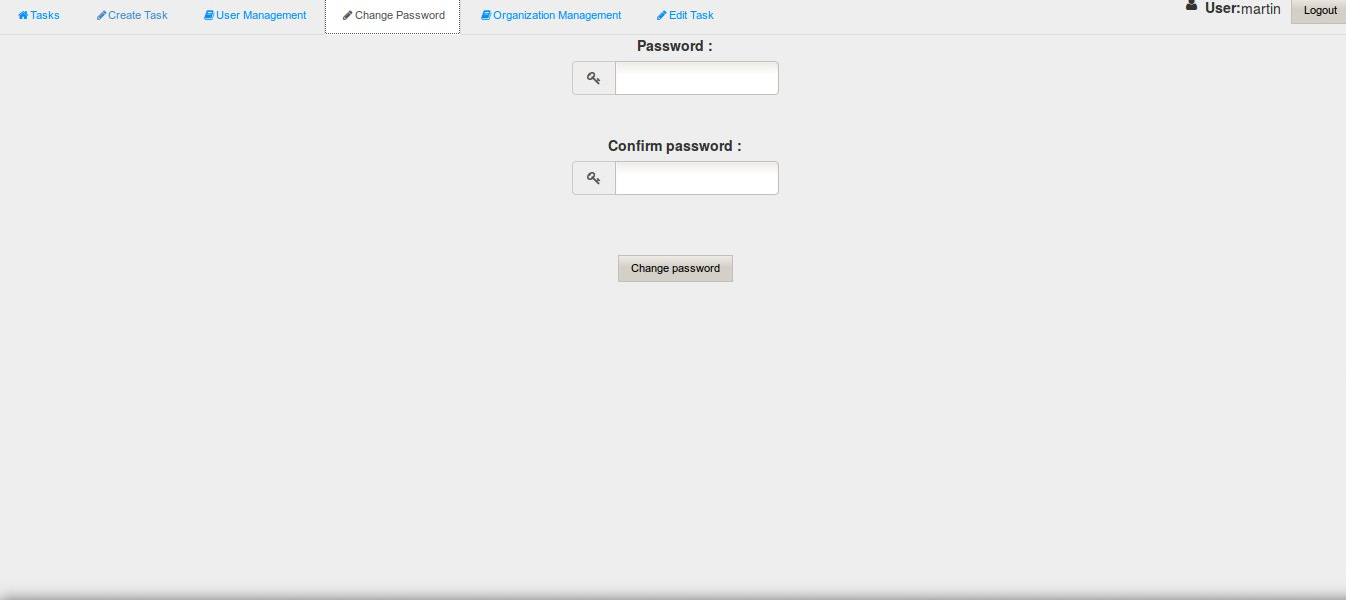
\includegraphics[scale=0.5]{page3.jpg} 
\caption{Zmena hesla}


\end{center}

\end{figure}

\begin{figure}[htb]

\begin{center}

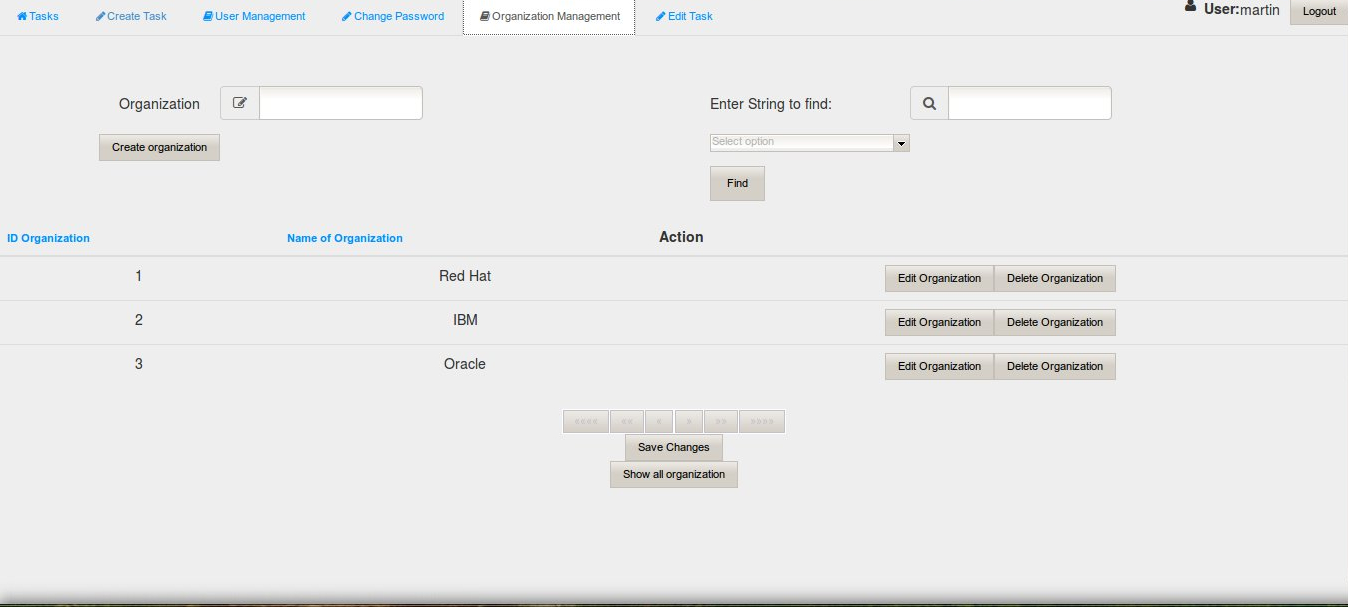
\includegraphics[scale=0.5]{page4.jpg} 
\caption{Spravovanie organizácií}


\end{center}

\end{figure}


}

\chapter{Dotazník}
{
	\section{Obsah dotazníka}
	{

	}


	\section{Grafické vyhodnotenie}
	{

	
	}


}

%\chapter{Konfigraèní soubor}
%\chapter{RelaxNG Schéma konfiguraèního soboru}
%\chapter{Plakat}

